\section{Model Component} \label{sc:model_component}
Based on the analysis of the problem domain, through the class diagram, event table and state charts, the model component of the system can be constructed.
\par
The model component, mentioned in \autoref{sc:component_architecture}, is constructed by first looking at the original class diagram from the problem domain (see \autoref{fig:FirstPDClassDiagram}). Then additional classes, attributes, and structures are added to support the mentioned events and the desired functionality of the system. The result is an updated class diagram, that contains attributes, operations, and additional classes.
\par
The customer has asked for a few extra functionalities, which cannot be extracted from the problem domain. These functionalities will be accommodated for in the following section and constitute with additions to classes, attributes, and structures.

\subsection{Additional classes}
Based on the events and desired functionality of the system, the following classes has been added to the class diagram. 


\subsubsection{Tag}
The \textit{Asset} class has the attribute 'Asset State' and the function 'Asset Acquired()', which can both be replaced by a class named \textit{Tag}. With the \textit{Tag} class, the \textit{Loan} will be obsolete, as the employee currently borrowing the asset can be tagged onto the asset. The \textit{Tag} class and tagging functionality have been requested by the customer. The \textit{Tag} class will contain information about the asset and will also be used to search through the assets. The tag has timestamps for its creation, last update, and deletion.

\subsubsection{Tag relation}
The \textit{Tag relation} class has been added to represent a connection between an asset and a tag, as an asset can have multiple tags related to it and a tag can be related to multiple assets.

\subsubsection{Department}
To more easily divide the assets and avoid cluttering the user with assets, a new class \textit{Department} has been added to the class-diagram. A department will have a name and contain a number of assets. An employee have a standard department, which they will be located in, when they open the application. The department can be change in the system by the employee, to see assets in another department, so the standard department will only be used as a starting point. A department also has timestamps for its creation and last update.

\subsubsection{Field}
To simplify the process of adding an asset to the system, only the relevant information should be available to fill in. To ensure that these attributes, without a clutter of irrelevant once, can be filled in intuitively, the \textit{Field} class is introduced.
\par
A field contains the following attributes:
\begin{itemize}
    \item Name
    \item Type of the input, which can be text, number, etc.
    \item Required, which is simply a boolean that defines if the field must be filled in to save the asset.
    \item \textit{Default value, which is the value of the field, if the tag on which it is placed is added to an asset, and the user does not change the value.}\newline This is only available on the fields added to a tag.
\end{itemize}
If the field is added to a tag, the field will appear on the asset as soon as it has been tagged with the given tag. When the field is added to a tag, the user can set a default value, which the field will take when an asset is tagged with the tag.
\par
Fields added directly to an asset does not give the opportunity to set a default value.

\subsubsection{Comment}
To better keep a history of the different events on an asset, the \textit{Comment} class has been introduced. A comment can be attached to an asset and contains the user adding the comment, the comment text, and timestamps for its creation, last update, and deletion.

\subsection{Attributes}
To ensure that every event and functionality is supported, the following attributes have been added to the classes from the class diagram in the problem domain.

\subsubsection{Asset attributes}
An asset has timestamps for its creation, last update, and deletion. The deletion time is used for soft deletion, which works as an extra step to avoid unwanted deletes. Soft deletion works by marking a asset with a deletion date in the database, instead of removing the element from the database, hereby allowing the asset to be recovered, if its accidentally deleted.

\begin{figure}[H]
    \centering
    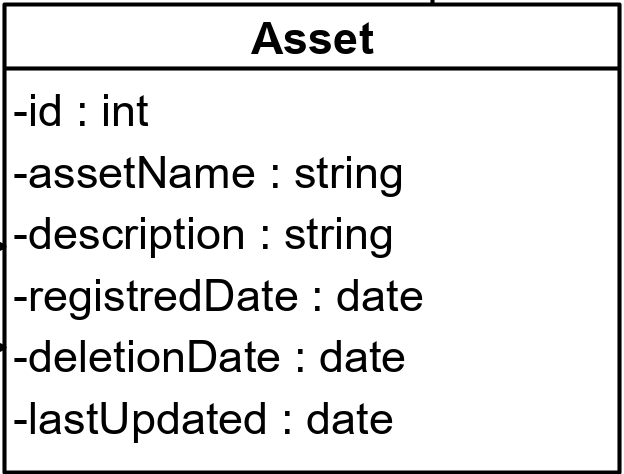
\includegraphics[width=0.5\textwidth]{figures/AssetClassOverview.PNG}
    \caption{Overview of the asset class}
    \label{fig:AssetClassOverview}
\end{figure}

\subsection{Structures}
The events and functions not completely supported by the previous mentioned classes and attributes will be achieved with the following structures of classes.

\subsubsection{An asset and a tag contains fields}
Both the \textit{Asset} and the \textit{Tag} classes aggregates the \textit{Field} class. An asset or a tag can contain multiple fields, but a field belongs to only one asset or one tag.

\begin{figure}[H]
    \centering
    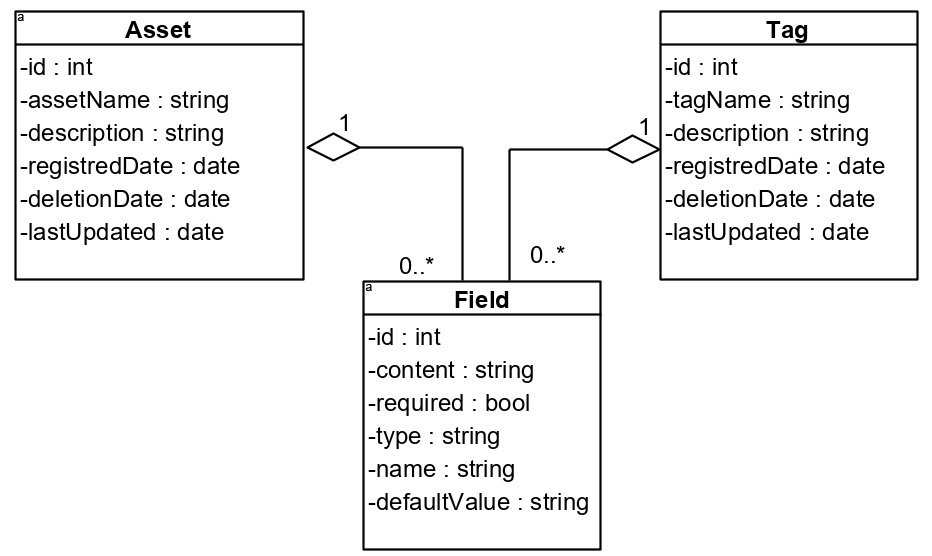
\includegraphics[width=0.8\textwidth]{figures/AssetFieldTagRelation.PNG}
    \caption{Overview of the asset class}
    \label{fig:AssetFieldTagRelation}
\end{figure}

\subsubsection{An asset contains comments}
An asset can be commented, which attaches the comment to the asset. An asset can have multiple comments, but a comment can only be attached to an asset.

\begin{figure}[H]
    \centering
    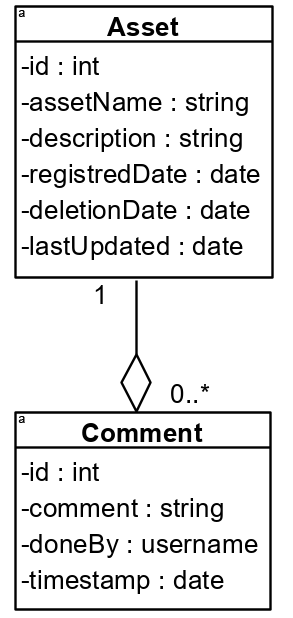
\includegraphics[width=0.2\textwidth]{figures/AssetCommentRelation.PNG}
    \caption{Overview of the asset class}
    \label{fig:AssetCommentRelation}
\end{figure}

\subsubsection{Tag relation between asset and tag}
Between the \textit{Tag} and \textit{Asset} classes is a many-to-many relation, which has been replaced by the class \textit{Tagged}. An asset can have multiple tag relations attached to it, as tags can be added to the asset dynamically. A tag does also have multiple tag relations connected to is, as a tag can be attached to multiple assets.

\begin{figure}[H]
    \centering
    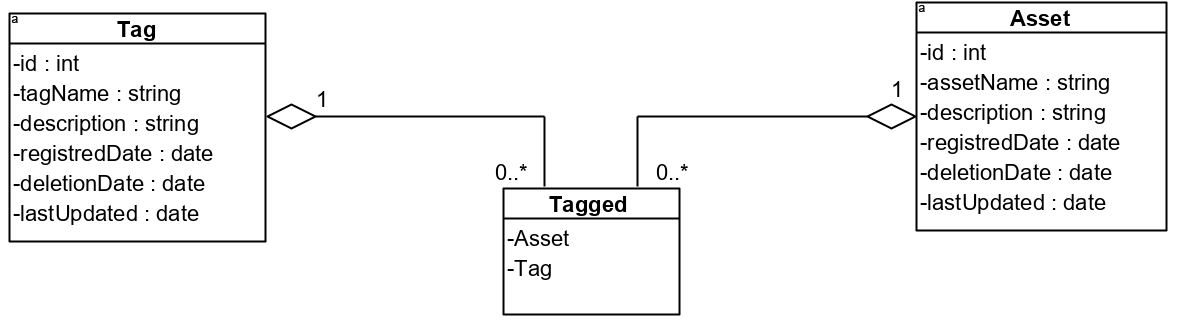
\includegraphics[width=0.8\textwidth]{figures/TagAssetRelation.PNG}
    \caption{Overview of the asset class}
    \label{fig:TagAssetRelation}
\end{figure}

\subsubsection{A department contains assets}
Assets are added to a department, as they are created. An asset belongs to exactly one department, and a department containing multiple assets.

\begin{figure}[H]
    \centering
    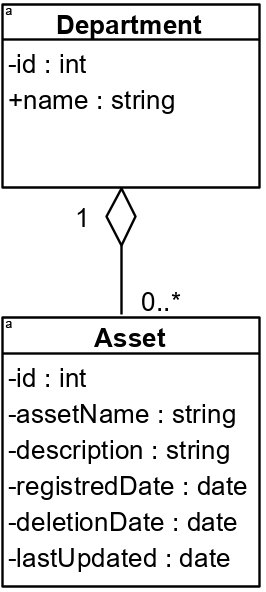
\includegraphics[width=0.2\textwidth]{figures/AssetDepartmentRelation.PNG}
    \caption{Overview of the asset class}
    \label{fig:AssetDepartmentRelation}
\end{figure}

\subsection{Updated class-diagram}
The additions mentioned above have added up to the following class-diagram, which will be the model component.

% Tags og andre ting skal introduceres inden dette afsnit
\begin{figure}[H]
    \centering
    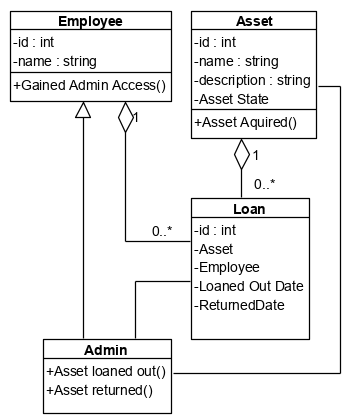
\includegraphics[width=0.8\textwidth]{figures/Model_ComponentV3.PNG}
    \caption{Class diagram for model component}
    \label{fig:ModelComponent}
\end{figure}
\todo[inline]{The model component class diagram must be updated to support the additions}

As illustrated in figure \ref{fig:ModelComponent} the classes now contain the attributes and operations described in the event table (table \ref{ssc:eventtable}) and state charts (section \ref{sc:behavoir}).